\chapter{Monte-Carlo Simulations of the SPM} 
\label{sec:numerics}
We now have numerical results for SPM systems using TRM analysis; however, this only allows us to study
relatively small systems. In order to study larger ones, we have used Monte-Carlo methods. In this
chapter, we will discuss the methods we used, the results they yielded and their meaning, with 
particular emphasis on what they tell us about the suspected transition between low and high-$\lambda$
behaviours.
\section{Numerical Simulations of Continuous-Time Markov Processes}
Here we will discuss the theory behind the Monte-Carlo methods used to simulated continuous-time Markov
processes. We will assume throughout that we have the computational means to produce pseudorandom
floating-point numbers in a way which which closely approximates the uniform real distribution over $(0, 1)$.
\subsection{Purpose of Monte-Carlo Methods}
We should first really describe what we mean by a Monte-Carlo method. In essence, Monte-Carlo methods
refer to numerical routines in which we attempt to characterise an unknown distribution, generated 
via known rules, by using
pseudorandom numbers in order to produce sample data which is hopefully faithful to the original 
distribution, at least in terms of the statistics we are trying to calculate. A good example of a
commonly-used Monte-Carlo method in Physics is the Metropolis-Hastings algorithm, which in its original
for is used to calculate statistics for equilibrium statistical mechanics systems.

In our situation, we wish to be able to mimic a continuous-time discrete-state Markov process.
As we saw in Chap.~\ref{sec:TRM}, the state space for a TRM system of size $L$ scales as
$\mathcal{O}(2^L$); thus we quickly run out of size if we try to consider exactly probability distributions, which correspond to
vectors in $\mathbb{R}^{L^2}$. We can, however, store individual configurations, which only occupy
$\mathcal{O}(L)$ space. Therefore, we need to find a way to produce trajectories through the discrete
state space which sample the actual space of system trajectories well enough to allow us to access the
statistics we want. Of course, there isn't a unique ``best'' way to do this. We have considered two
contrasting methods, which differ primarily in the way in which they convert the original continuous 
time into discrete steps which we can use in an algorithm.

\subsection{Evenly-Spaced Timesteps} \label{sec:evenTimesteps}

If we wished to numerically approximate an ODE system, one might use the Euler forward or 
Runge-Kutte methods. These both involve discretising time simply by dividing it into evenly-sized
pieces, and then converting the ODE into a discrete form by using finite differences to
approximate derivatives. We need to be careful to choose a small enough timestep for
the approximation to the derivative to remain good, but otherwise it is a very simple and 
effective approach.

We can do a very similar technique with continuous time Markov processes. In our SPM system,
if we ignore the boundaries, there are two rates, $1$ and $\lambda$, and our system is 
homogeneous. Let us represent the system with a binary array of length $L+2$, with $L$ sites for the bulk
and a site each representing the boundaries. Therefore, in order to simulate the action of the SPM as
defined in <reference to appropriate section in
introduction>, we can use the following recipe:
\begin{enumerate}
 \item \textbf{START}. Advance time by $\Delta t$. Pick a site, which we will call
 Site,
 (of which there are $L+2$) at random. If the site chosen is one of the boundaries with density $\rho$,
 reset the site to be occupied with probability $\rho$ and unoccupied with probability $1-\rho$.
 \item If Site is occupied, pick one of the two adjacent sites, which we will call Target, at random with equal probability.
 This will be the site we attempt to move into. If it is not, go back to \textbf{START}.
 \item \textit{If Site is not on the boundary}: If Target is occupied, go to \textbf{START}. Otherwise, consider the other adjacent site,
 which we will refer to as Rear. If Rear is empty, move the particle in Site into Target 
 randomly with
 probability $\frac{1}{1+\lambda}$; otherwise, move the particle with probability
 $\frac{\lambda}{1+\lambda}$. Return to \textbf{START}. 
 \newline \textit{If Site is on the boundary}: If Target is outside the system, go to \textbf{START}.
 If Target is occupied, go to \textbf{START}. Assign an occupation value for Rear randomly, occupied
 with probability $\rho$, unoccupied with probability $1-\rho$, where $\rho$ is the density of the relevant
 boundary. Now, if Rear is empty, move the particle in Site into Target 
 randomly with  probability $\frac{1}{1+\lambda}$; otherwise, move the particle with probability
 $\frac{\lambda}{1+\lambda}$. Return to \textbf{START}.
\end{enumerate}
We define $\Delta t$ via 
\begin{equation}
 \Delta t = \frac{\tau_0}{L (1+\lambda)}.
\end{equation}
In terms of the algorithm's correctness at producing reasonable trajectories, we simply need note that
the rates at which particular transitions should occur are in the correct proportions, and that the boundaries result in the correct densities in equilibrium;
then, we just need
to verify that the rate at which free particles move is the correct one in absolute terms, which it is,
and we're done. 

For Monte-Carlo methods, we generally rate their performance by the amount of computational
power required to explore a given amount of the probability space. In methods in which we
are exploring this space by advancing though time (and invoking ergodicity) we desire methods
which move us quickly through time whilst maintaining good sampling and performing little computation.

The advantage of this method is that it is very simple; thus, there aren't too many opportunities
for error when writing the code, it uses very little memory (all calculations can be performed
in-place), and each iteration should be very fast as there are very few overheads. It should also
produce trajectories which are good samples of the original probability distribution we are 
trying to replicate.


If $\lambda$
is close to $1$, the probability of rejection (i.e. a step which results in no overall change to
the system) is $\sim\frac{1}{2}$, and this is the situation in which the algorithm really shines; similarly
it also performs well for large or small $lambda$ if the system density is very high or very low
respectively. For extreme $\lambda$ in general however, performance drops off considerably, as
we are often performing lots of calculations and advancing time very little, and thus not seeing
much of the distribution simply because we aren't moving much.

We could have made this code marginally more efficient by making the more likely moves certain, and
correspondingly adjusting the timestep size $\Delta t$ to account for this; however, this only
improves efficiency by a factor of around $2$ , whilst making the code more complicated, so as
we only used this method to verify the results of our main code we didn't bother.
It is possible for us to get
around this issue by advancing time in a variable fashion, although this comes at the cost of
a little more computation per iteration.

\subsection{The N-Fold Way, or Gillespie Algorithm} \label{sec:nFoldWay}
A popular way to produce trajectories for a continuous-time Markov process is the N-Fold Way, also known as
BKL, or Gillespie Algorithm~\cite{Bortz1975, Prados1997, voterKMC}. It evolves us through time as follows:
\begin{enumerate}
 \item \textbf{START}: Make a list of all states which can be transitioned to in a single move from the 
 current state, and the associated rates at which this occurs.
 \item Weight each successor state by the transition rate into it, and then select a successor state by
 random selection from a uniform distribution over the weighted possible successors. Change the system
 state to the chosen successor. \label{weightingChoose}
 \item Now advance time by an increment chosen from an exponential distribution whose decay rate 
 is the sum of all of the rates of the possible transitions to a successor. Go back to \textbf{START}. \label{timestepChoose}
\end{enumerate}
Now we just need to supply the rates <from introduction> that define the SPM, along with some additional rates describing processes at the boundary. Specifically, we use the method described 
in~\ref{sec:CTMPBoundaries} to do this, whereby we have a double layer of ``blinking'' boundary sites
and sites in the internal layer undergo the same transitions as in the bulk. However, unlike in our TRM
calculations, we should not set the incoming and outgoing rates to be extremely high, as then these rather
trivial processes come to dominate the calculation and cause the timesteps to be on average extremely small, wasting our computing time. Instead, we set them to
be proportional to the geometric mean of $1$ and $\lambda$, and thus in the language of~\ref{eq:blinkRates}
this corresponds to setting $B_0 = \sqrt{\lambda}$. This way the boundaries refresh often, but not too
often, and should still act as suitable reservoirs.

We will get into the fine details about how the software we use implements KMC in Sec.~\ref{sec:kmcLib}.
Let us instead discuss how we obtain the required probability distributions using the uniform distribution
on $(0, 1)$, $U(0, 1)$:
\begin{itemize}
 \item We can randomly choose the successor state required in step~\ref{weightingChoose} by
 creating a list of weighted partial sums. If the transition rate from the current state the $i^\mathrm{th}$
 potential successor state is $k_i$, then let us define $k_\mathrm{Tot.} = \sum_{i}^n$, where $n$ is the
 number of potential successors. Create the list of partial sums via $s_i = \sum_j^i k_j$, then generate
 the random number $u = r k_\mathrm{tot}$ where $r$ is drawn from $U(0, 1)$. We can then use a binary
 search to find $i: s_{i-1} \le u \le s_i$, and then this $i$ indicates the successor state which has been
 chosen. This process is illustrated more visually in Fig.~\ref{fig:weightChoice}.
 \item In step~\ref{timestepChoose}, we need to generate random numbers in an exponential distribution
 with decay rate $k_\mathrm{tot}$. We can do this by generating $r$ from $U(0, 1)$, and then $w = -\frac{1}{k_\mathrm{tot}} \log{r}$
 follows the desired distribution.
\end{itemize}
\begin{figure}[h!]
 \caption[Illustration of the method for choosing successor states in the n-fold way.]{\label{fig:weightChoice} 
 An illustration of the suggested method for choosing a successor state in the n-fold way. Reproduced
 from~\cite{voterKMC}.
 }
  \begin{center}
 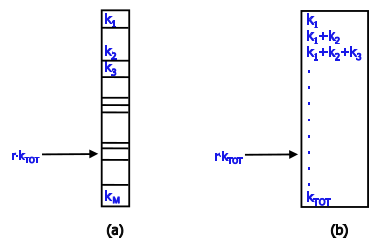
\includegraphics[width=0.7\textwidth]{numerics/images/nFoldWayRates}
  \end{center}
\end{figure}

I will defer to Voter (see in particular Sec. 5 of~\cite{voterKMC} for the ``proof of correctness'' of the
method. The primary advantage of this method is that we are certain to advance time every step, so we are
not potentially
``wasting'' steps as
when we use even 
timestepping; this comes at the cost of having to compute which transitions are possible from the current
state. For our SPM, a given state has $\mathcal{O}(L)$ possible transitions, thus the time complexity
of a single timestep is $\mathcal{O}(L)$; note that our method with evenly-spaced timesteps has constant
time complexity, but the size of each timestep scales as $\mathcal{O}(L^{-1})$; thus we're not actually
losing as much as it appears by using variable timesteps. Furthermore, there is the possibility that the
process by which we calculate which transitions are possible could be performed in parallel, and so
the walltime cost of a single timestep in the n-fold way can end up comparatively cheap. The process of
choosing a successor state once the options are found involves performing the equivalent of a search, and
therefore takes $\mathcal{O}(\log{L})$ time and so should be insignificant.


\section{Implementation of Monte Carlo Methods}
\subsection{Our Implementation of a Metropolis-Hastings Algorithm with Evenly-Space Timesteps}
We have written a Fortran code which implements the algorithm in Sec~\ref{sec:evenTimesteps}. This is
stored in <location of code>. This programme initialises the system to have a particle density
equal to the average of the two desired boundary densities, and then proceeds in a manner extremely
faithful to the simple accept/reject algorithm.


\subsection{\texttt{KMCLib}} \label{sec:kmcLib}
The vast majority of our Monte-Carlo calculations have been performed using the n-fold way, described in
Sec.~\ref{sec:nFoldWay}. This is implemented for continuous-time Markov processes on crystalline lattices
(of which the SPM is an example) in a software package called \texttt{KMCLib}, documented 
at~\cite{leetmaa2014KMCLib} developed by Dr Mikael Leetmaa.

\texttt{KMCLib} is a Python-wrapped C++ package. This means that the frontend, where one specifies the
system to be simulated, the data to be recorded, and how the simulation is run, is written in a Python
script; then, when this script is run, it executes C++ code in order to represent the system and
actually carry out the desired operations. Furthermore, \texttt{KMCLib} can perform calculations in
parallel if so desired. Whilst there exist examples~\cite{hoffmann2014kmos, spparks} of kinetic
Monte-Carlo codes other than \texttt{KMCLib}, we chose to use that one due to our familiarity with all
of the languages involved, and preference for a Python frontend.

Of course, setting up different calculations which vary different parameters or measure different things
require different scripts. Going through every script we wrote individually would cause this thesis
to be around twice as long and three times more dull; therefore we have instead chosen to focus
upon a single set of codes designed to perform a particular calculation, which we have annotated and 
included here <location>; the intention is that a reader wishing to reproduce any of our results could do
so by performing a few simple modifications to the code listed there. A more comprehensive codebase is
stored at <location>, but this is sparsely annotated working code, and so might not be very helpful.

The exemplary code which actually interfaces directly with \texttt{KMCLib} is contained within 
\texttt{concFlow.py}. This script takes in several command line inputs. These provide the parameters for
a simulation of the SPM, with the desired value of $\lambda$, system size and boundary conditions. It 
then sets up the representation of the system configuration and the means to enumerate possible
transitions and their associated rates, as is necessary to implement the n-fold way.
The initial configuration is generated by randomly inserting particles into the system until its density
is equal to $\frac{1}{2}\left(\rho_0 + \rho_L \right)$; we then perform $N_{\mathrm{eq}}$ KMC steps in order to 
equilibrate the system (in case the initial configuration we chose was highly deviant from the norm
for the prescribed parameters). The actual measurements are performed by time-averaging values for system
quantities (e.g. the number of particles entering the system at one end) over $N_{\mathrm{meas}}$ steps,
relaxing the system (in other words, performing steps but taking no measurements) for $N_{\mathrm{req}}$ steps,
and then repeating this process $N_{\mathrm{pass}}$ times. This way, we can generate $N_{\mathrm{pass}}$ time-separated 
observations of, say, the total current through the system, and because we are relaxing the system 
between measurement runs we should not have to worry too much about the results being unduly correlated
with each other, (assuming we set $N_{\mathrm{req}}$ high enough).
Thus, we supply \texttt{concFlow.py} with the following parameters as 
command line inputs:
\begin{enumerate}
 \item The particle reservoir concentration at one end of the domain, $\rho_0$.
 \item The particle reservoir concentration at the other end of the domain, $\rho_L$.
 \item The value of $\lambda$ to use in the simulation.
 \item The system size, $L$.
 \item The interval between measurements performed by the analysis
 routines, $N_{\mathrm{anal}}$. This should be set to $1$ in order to measure the current.
 \item The number of equilibration steps, $N_{\mathrm{eq}}$.
 \item The number of analysis steps per pass, $N_{\mathrm{meas}}$.
 \item The number of reequilibration steps per pass, $N_{\mathrm{req}}$.
 \item The total number of passes, $N_{\mathrm{pass}}$, which give separate
 sets of observations, performed during this calculation.
 \item A timescale, $\delta t$, which indicates how often to evaluate,
 and to what accuracy to record times, when measuring the number of 
 particles in the system. This should probably be small compared to the expected KMC timestep size.
\end{enumerate}

In terms of the output of the code, it produces a short file summarising the input parameters,
some trajectory dump information (usually redirected to \texttt{/dev/null} in order to save hard
memory, which is often in short supply), as well as data taken by measurement routines. We nominate,
from a suite of possible routines, which measurements we would like it to take during analysis phases.
Note that in our calculations, we do not consider any quantity's value on during particular KMC steps;
rather, we always average our quantities over some amount of time. This is partly because some of the
quantities we are interested in do not really have any value during a single timestep (e.g. the flux of
particles through one of the boundaries), and also because the amount of time spent in particular
configurations could potentially vary wildly between configurations. The amount of time spent in a
particular configuration in the n-fold way is drawn from an exponential distribution with decay rate
$k_{\mathrm{tot}}$, as we saw in Sec.~\ref{sec:nFoldWay}; thus, one could easily imagine a
situation in which the transition time varies wildly. For example, say we have a system with very low 
$\lambda$. If this system was quite full, there would be few transitions possible, and those possible
transitions would likely occur with low rates, therefore the kmc timesteps would tend to be very long.
However, later during the same simulation we could find ourselves in a situation where the system is
less full, and so more transitions can occur, and generally with much higher rates, leading to much
shorter timesteps. Thus, we shouldn't really treat particular quantities derived from these 
configurations with an equal footing, as the amounts of time the system spends in each are so very 
different.

The precise nature of our time-averaging depends a little on the measurement in question. The types
of measurements we usually perform are the following, where $T$ is the total time elapsed during
our $N_\mathrm{anal}$ step measurement run:
\begin{itemize}
 \item \textbf{Current} We count the total number of particles which enter or leave a given boundary
 over the course of the measurement run. Let the number of particles entering and 
 exiting at the $0$ boundary be $u_0$ and $w_0$ respectively, and likewise for the $L$ boundary with
 $u_L$ and $w_L$. Then
 \begin{equation}
  J = \frac{u_0+w_L-u_L-w_0}{2T}
 \end{equation}
should be a good estimate of the total current through the system during that time period.
\item \textbf{Block Size Distribution} In one dimension, we can look at a configuration and count how
many contiguous runs (``blocks'') of particles there are of different sizes (e.g. size 1 means a single
particle sandwiched between adjacent vacancies). We can find the distribution of block sizes, weight it
by the length of the associated kmc timestep, and then add this to a running total. If we do this over
our $N_\mathrm{meas}$ analysis steps and then normalise, we can build a histogram of the block sizes
during that time period.
\item \textbf{Particle Density} Similarly, we can count the total number of particles in the system,
weight it by the length of the kmc timestep, and then use this to build another histogram of the
system particle density. By keeping track of particles entering and leaving the system, it would be
possible to code this very efficiently to take $\mathcal{O}(1)$ time; however, as our routine to detect
block sizes scans through the system and counts as it goes along, we have just opted for a simple
$\mathcal{O}(L)$ scan of the whole system for our density measurement as well.
\end{itemize}
Using these analysis routines, we can generate time-averaged values for particle density histograms,
the block size distribution and the current. By calculating $N_\mathrm{pass}$ separate instances of 
these observables, we get $N_\mathrm{pass}$ samples from the relevant distributions, and from there
we can probe the statistics of these variables.


\subsection{Managing \texttt{KMCLib} Calculations in Parallel} 
Of course, it is one thing to have a code which can run on a laptop to produce the output of a 
particular simulation over the course of a day. It is quite another undertaking to run thousands of
separate calculations in order to map out parameter spaces and compute derived quantities such as the
diffusion coefficient. 

We have been running our calculations on Edinburgh University's \texttt{Eddie3} computing cluster.
This machine does not boast the high level of processor interconnection density of \texttt{ARCHER}
or the extremely high working memory of \texttt{DiRAC}; however, for the purposes of our calculations
it turns out that we need neither. The KMC algorithm only stores a single state of the system under
simulation at any given time, therefore its space complexity only scales as $\mathcal{O}(L)$.
Furthermore, whilst \texttt{KMCLib} can be run in parallel mode in order to take advantage of
a multithreaded environment, this isn't actually an advantage when we wish to run very large numbers
of separately-parametrised calculations, as the total amount of CPU time required remains the same,
whilst incurring additional overheads associated with parallelism.
Therefore, we have used a single-threaded environment for all of the calculations featured in this
thesis.

In order to set up a batch of calculations, we use the following procedure, implemented by the codes
stored in \texttt{kmc/1d/} within <location>:
\begin{enumerate}
 \item Created a batch of input files, in the subdirectory \texttt{jobInputs/}. In our setup, we
 require that files titled
 \texttt{testInput.}$i$ are generated, with $i \in [1, n]$ where $n$ is the total number of 
 calculations to be performed. These input files are typically generated by a code such as 
 \texttt{lambdaFlucCreator.py}, and typically the parameters which determine the overall structure
 of the system (e.g. $L$, the system size) will be held constant across calculations, whilst
 parameters such as the stickiness or the boundary densities will be varied between them. These input files contain a single line of code, which will be appended to $python $ and called in the command line.
 \item In order to actually perform the calculations, we submit them as \texttt{gridengine} batch
 jobs. We then run the script \texttt{kmcSubmit.sh}, which submits the nominated tasks whose input
 files are in \texttt{jobInputs/}, using the scripts \texttt{kmcJobArray.sh} and 
 \texttt{initKmc.sh} for intermediate steps. \texttt{kmcSubmit} is also the place where we specify
 calculational parameters, such as maximum memory usage, maximum runtime, etc; these will be taken
 into consideration by \texttt{gridengine} when it comes to scheduling these calculations, so it
 is important that the maxima be relatively tight upper bounds, otherwise the calculation priority
 will be extremely low, assuming that the cluster in question is being simultaneously for many other
 calculations.
 \item The jobs will then be executed, in their own time. The results will be placed in the location
 nominated by the input files.
 \item Once the run is complete, and the data has been saved, we are then ready to process it into a
 more useful format, in our case a data file which can be interpreted by Mathematica, the programme
 we used for most of our analysis and graphing. This is done using a script such a 
 \texttt{lambdaPostProc}. Note that such
 a script needs to be able to handle the fact that data may not be produced for some of the 
 calculations (around 5\% in our experience). The most likely source of the
 problem seems to be an issue with type conversion between Python and C++, which only seems to 
 become a significant issue in larger calculations.
\end{enumerate}
Note that throughout our calculations, we have stored data in a human-readable format, instead of
in a more compressed binary format. This is because we believe that the benefit of having a 
human-readable format, and therefore a much greater ability to look through data and check the 
output, outweighs the associated memory cost (around a factor of $10$ or so), 
especially given that any memory reduction attained due to such a format change wouldn't change
what was feasible in terms of what we can afford to store.


\section{1D Calculation Results}
\subsection{Calculational Choices}
\subsection{Flow Patterns}
\subsection{Current}
\subsection{Density}
\subsection{Diffusion Coefficient}

\section{2D Calculation Results}
\subsection{Calculational Choices}
\subsection{Results}

\section{Conclusions}
